\documentclass[twoside,a4paper,openany,12pt]{book}
%%\documentclass[twoside,a4paper,12pt]{article}
%\documentclass[twoside,a4paper,openany,12pt]{report}

%% Document has convention that only first letter of chapters,
%% sections is capitalized. Do the same for automatic sections
\renewcommand\listfigurename{List of figures}
\renewcommand\listtablename{List of tables}

%% Convenient way to specify margins
\usepackage[a4paper,top=2.5cm,bottom=2.5cm,inner=2.5cm,outer=2.5cm]{geometry}

%% Relative font sizes
\usepackage{relsize}

%% Nicer fonts
\usepackage{pslatex}

\usepackage{linegoal}

%% Color definitions
\usepackage{color}
\definecolor{MyLightRed}{rgb}{1,.8,.8}
\definecolor{MyCodeboxColor}{rgb}{.9,.9,.9}
\definecolor{MyLightBlue}{rgb}{.8,.8,1}
\definecolor{MyQuoteColor}{rgb}{0,.6,0}
\definecolor{MyLightMagenta}{rgb}{1,.2,1}

%% For landscape pages printed, but rotated on screen
\usepackage{pdflscape}

%% Including figures and other graphics
\usepackage{graphicx}

%% Rotated images etc
\usepackage{rotating}

%% Author-year citations
\usepackage[authoryear]{natbib}

%% Subfigure environment
\usepackage{subfigure}

%% Conditional sections
\usepackage{ifthen}

%% URLs
\usepackage[obeyspaces]{url}

%% SI units
\usepackage[abbreviations]{siunitx}

% Command to get a tilde which prints as an ASCII tilde in PDFs,
% needed to allow copying text and pasting into a command window or
% editor
\newcommand{\mytilde}{\texttildelow}

%% For tables align on decimal point
\usepackage{dcolumn}
\newcolumntype{d}{D{.}{.}{-1}} % centre on decimal place

%% Long tables
\usepackage{supertabular}

\usepackage{fancyhdr}

%% Alternative to verbatim. Can be used for defining new environments
\usepackage{fancyvrb}
%% A command to include Matlab files (verbatim). Surrounded with a
%% frame and smaller font size than normal. Must be defined before
%% underscore package because the custom command must be listed in
%% \UnderscoreCommands
\CustomVerbatimCommand{\IncludeMatlabFileVerb}{VerbatimInput}{frame=single,fontsize=\relsize{-1}}
\CustomVerbatimCommand{\IncludeShellFileVerb}{VerbatimInput}{frame=single,fontsize=\relsize{-1}}

%% Include Matlab file verbatim and attach it for the user to download.
\newcommand{\IncludeMatlabFile}[2]{\IncludeMatlabFileVerb{#1}%
  \attachfile[mimetype=text/plain,description=#2]{#1}}

%% Include shell file verbatim and attach it for the user to download.
\newcommand{\IncludeShellFile}[2]{\IncludeShellFileVerb{#1}%
  \attachfile[mimetype=text/plain,description=#2]{#1}}


%% Have floats on subsequent page, not miles away.
\usepackage{flafter}

\usepackage{marvosym} % for \Info
\usepackage{keystroke} % for keyboard symbols


% Load the underscore package as fixes the problem of copying and
% pasting text with underscores; previously underscores were converted
% to spaces, but they matter for code! Need to protect certain
% commands which take input which has underscores (see underscore
% package for details)
\newcommand{\UnderscoreCommands}{%
  \do\VerbatimInput
  \do\BVerbatimInput 
  \do\IncludeMatlabFileVerb
  \do\IncludeShellFileVerb
}
\usepackage[strings]{underscore}

%% Include these packages last!
\usepackage[bookmarksnumbered=true,
bookmarksopen=true,
bookmarksopenlevel=0,
colorlinks=true,
linkcolor=blue,
citecolor=blue,
urlcolor=blue,
unicode=true,
pdftitle={AuroraWatchNet magnetometer manual}]{hyperref}

%% Attach files to PDF document. Set the default options we want.
\usepackage{attachfile2}
\attachfilesetup{icon=Paperclip}

%% Upright quotes, essential for quoting for Matlab code!
\usepackage{upquote}

%% A command for the return key
\newcommand{\myreturn}{%
  \keystroke{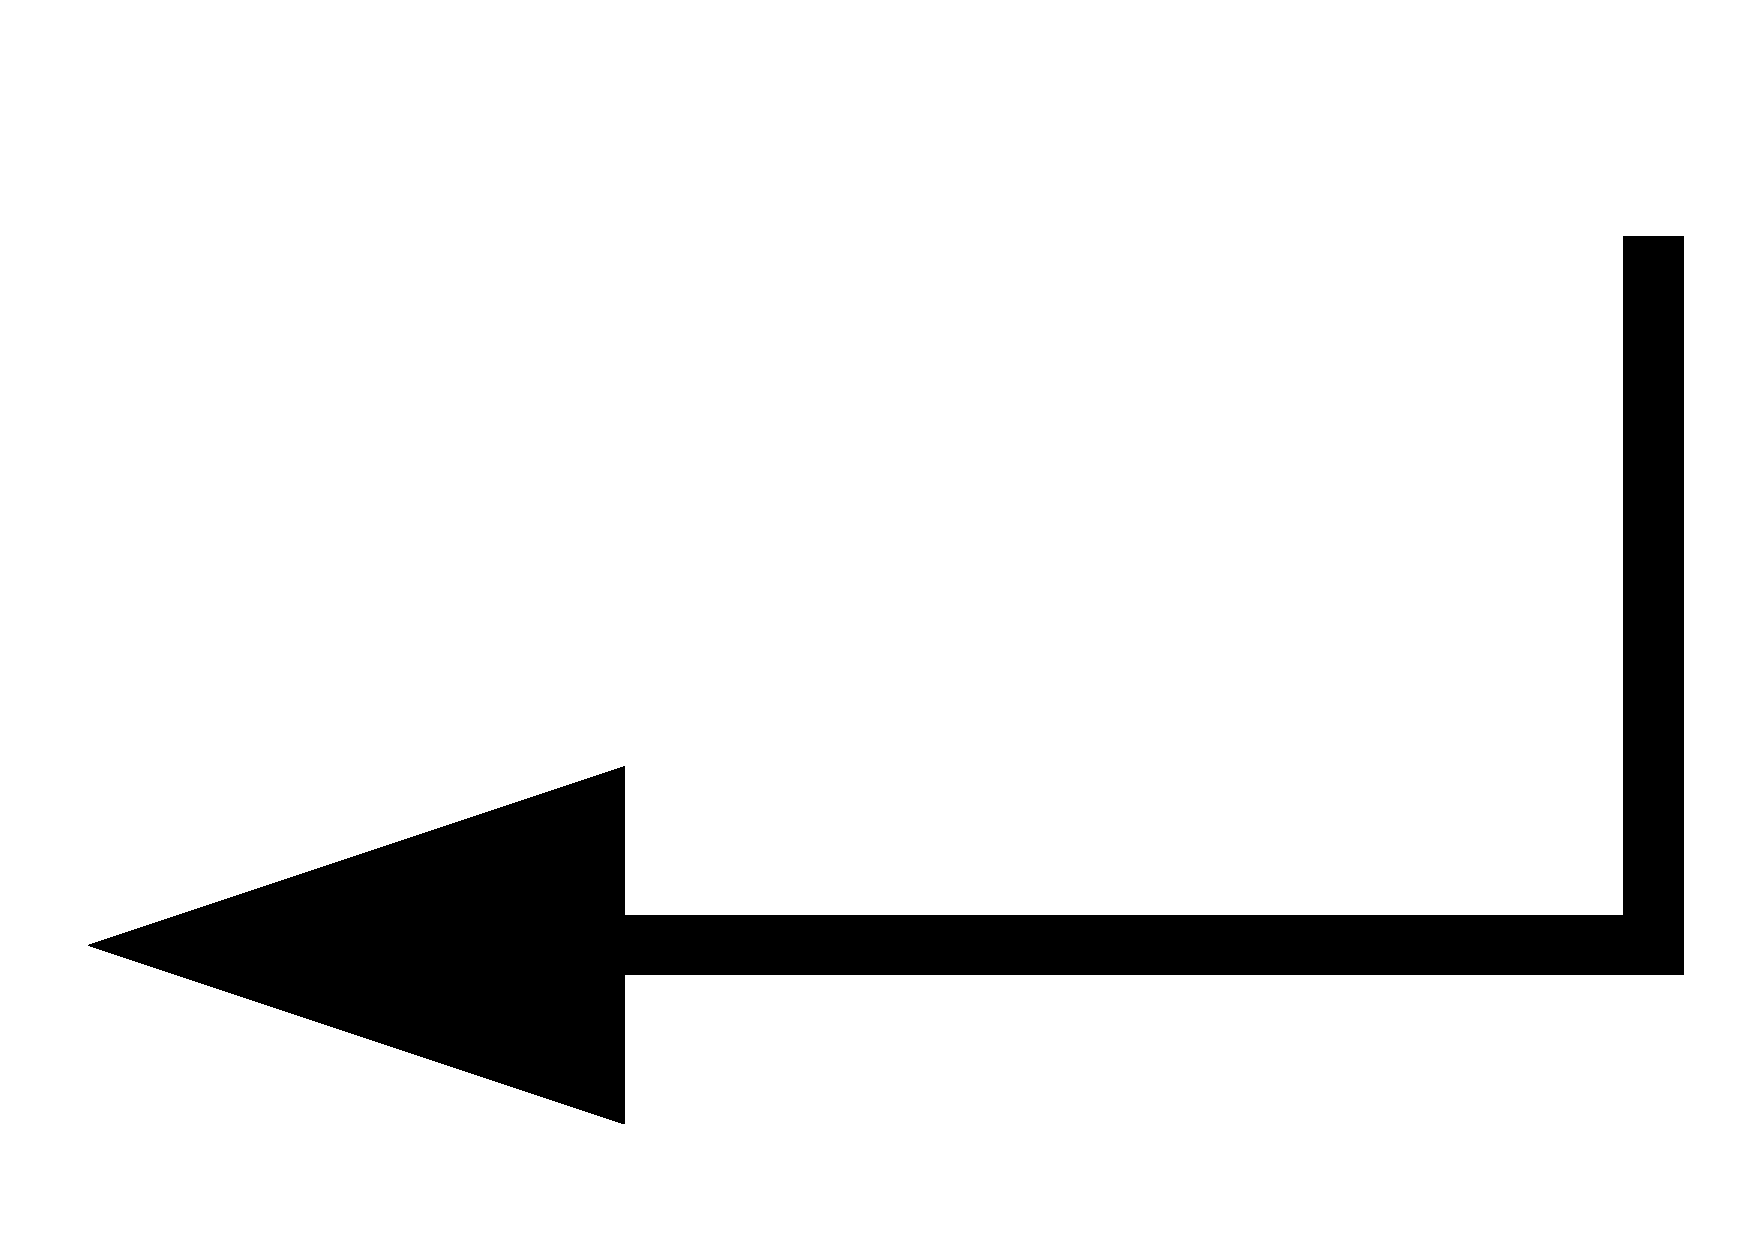
\includegraphics[width=1em]{images/return-symbol}}}

%% Change how subfigures are labelled
\makeatletter
\renewcommand{\@thesubfigure}{\figurename~\thefigure\alph{subfigure}: }
\renewcommand{\thesubfigure}{\alph{subfigure}}
%%%\renewcommand{\p@subfigure}{\alph{subfigure}}
\makeatother

% No indents at start of paragraph, but paragraphs have blank lines
% between them
\setlength{\parindent}{0pt}
\setlength{\parskip}{2ex} 


%% \filename allows for _ but otherwise is formatted identically to
%% code. If using tildes (~) then use \mytilde command, inside
%% \texttt. Use the url package's command to define this, that way
%% hyperref doesn't see it as a hyperref!
\DeclareUrlCommand\filename{\urlstyle{tt}}
\newcommand{\email}[1]{\href{mailto:#1}{#1}}
\newcommand{\ccThreeUrl}{http://creativecommons.org/licenses/by-sa/3.0/}

%% Environment variables. Like \filename but prepends a $
\DeclareUrlCommand\envVar{\def\UrlLeft{\$}\urlstyle{tt}}
\DeclareUrlCommand\dosEnvVar{\def\UrlLeft{\%}\def\UrlRight{\%}\urlstyle{tt}}

\newcommand{\code}[1]{\texttt{#1}}
\newcommand{\username}[1]{\texttt{#1}}
\newcommand{\piUser}{\username{pi}}
\newcommand{\rootUser}{\username{root}}

%% Use for menu selections etc
\newcommand{\myquote}[1]{\textcolor{MyQuoteColor}{\textsl{#1}}}

%% Define our own keypress command, based on keystroke
\newcommand{\keypress}[1]{\keystroke{#1}}

%% Units
%%\newcommand{\units}[2]{\mbox{\ensuremath{#1}\,#2}}
%%\newcommand{\dB}[1]{\mbox{\ensuremath{#1}\,dB}}
\newcommand{\dB}[1]{\SI{#1}{dB}}
\newcommand{\inch}[1]{\mbox{\ensuremath{#1}''}}
\newcommand{\kHz}[1]{\mbox{\ensuremath{#1}\,kHz}}
%\newcommand{\metre}[1]{\mbox{\ensuremath{#1}\,m}}
\newcommand{\km}[1]{\mbox{\ensuremath{#1}\,km}}
%% \newcommand{\MHz}[1]{\mbox{\ensuremath{#1}\,MHz}}
\newcommand{\MHz}[1]{\SI{#1}{\mega\hertz}}
\newcommand{\volt}[1]{\mbox{\ensuremath{#1}\,V}}
\newcommand{\bit}[1]{\mbox{\ensuremath{#1}\,bit}}

%%\newcommand{\degrees}[1]{\ensuremath{#1^\circ}}

\renewcommand{\textohm}{\ensuremath{\Omega}}
\newcommand{\ohm}[1]{\SI{#1}{\ohm}}
\newcommand{\kohm}[1]{\SI{#1}{\kilo\ohm}}


\newcommand{\pF}[1]{\SI{#1}{\pico\farad}}
\newcommand{\nF}[1]{\SI{#1}{\nano\farad}}
\newcommand{\uF}[1]{\SI{#1}{\micro\farad}}

\newcommand{\uH}[1]{\SI{#1}{\micro\henry}}

%% Some simple abbreviations  
\newcommand{\ie}{i.e.}
\newcommand{\eg}{e.g.}
\newcommand{\etal}{\latin{et al.}}
\newcommand{\etc}{etc.}
%% Have warnings printed in light red box, with each item using a
%% STOP sign as a bullet
\newenvironment{warninglist}{%
  \begin{list}{\Stopsign}{}}{%
    \end{list}}
\newcommand{\warningbox}[1]{\noindent%
  \colorbox{MyLightRed}{\parbox{\textwidth}{%
      \begin{warninglist}\item #1\end{warninglist}}} \newline}

%% Have help information printed in light blue box, with each item using an
%% information sign as a bullet
\newenvironment{helplist}{%
  \begin{list}{\Info}{}}{%
    \end{list}}
\newcommand{\helpbox}[1]{\noindent
  \colorbox{MyLightBlue}{\parbox[l]{\textwidth}{%
      \begin{helplist}\item #1\end{helplist}}} \newline}

%% Verbatim-like environment for code.
\DefineVerbatimEnvironment{Code}{Verbatim}%
{frame=single,commandchars=\\\{\}}
\DefineVerbatimEnvironment{Cmd}{Verbatim}%
{frame=single,framesep=5mm,commandchars=\\\{\}}
% {frame=single,label=\linuxLogo,framesep=5mm,commandchars=\\\{\}}
\DefineVerbatimEnvironment{LinuxCmd}{Verbatim}%
{frame=single,framesep=5mm,commandchars=\\\{\}}
% {frame=single,label=\linuxLogo,framesep=5mm,commandchars=\\\{\}}
\DefineVerbatimEnvironment{WindowsCmd}{Verbatim}%
{frame=single,framesep=5mm,commandchars=\\\{\}}
% {frame=single,label=\windowsLogo,framesep=5mm,commandchars=\\\{\}}

%% \DefineVerbatimEnvironment{Cmd}{LinuxCmd}{}


\newcommand{\todo}[1][]{\fcolorbox{magenta}{MyLightMagenta}{\mbox{\textcolor{black}{TO DO\ifthenelse{\equal{#1}{}}{}{: #1}}}}}

\newcommand{\figscale}{1.0}

%% Have subsubsections numbered
\setcounter{secnumdepth}{5}
\setcounter{tocdepth}{5}


\newenvironment{buildorder}{%
  \begin{enumerate}%
    \setlength{\itemsep}{0pt}%
    \setlength{\parskip}{0pt}}%
  {\end{enumerate}}

\begin{document}

\title{AuroraWatchNet magnetometer manual}
\author{Steve Marple, \\
Lancaster University.}
\date{\today}
\maketitle
\thispagestyle{empty}
\frontmatter
\pagestyle{headings}

% \clearpage  
% \phantomsection  
% % \thispagestyle{empty}
\chapter{Licence}
This document is made available under the \href{\ccThreeUrl}{Creative
  Commons Attribution-ShareAlike 3.0 Unported Licence}.

\begin{center}
\href{\ccThreeUrl}{\includegraphics{images/by-sa}}
\end{center}

\clearpage  
\phantomsection  
\addcontentsline{toc}{chapter}{\contentsname}  
\tableofcontents

\newpage
\phantomsection  
\addcontentsline{toc}{chapter}{\listfigurename}  
\listoffigures

%% -----------------------------
\newpage
\phantomsection  
\addcontentsline{toc}{chapter}{\listtablename}  
\listoftables


%% List of abbreviations. Include all useful ones. Those which are not
%% used are not included in the table.

\abbrev{\adc}{ADC}{analogue to digital converter}
\abbrev{\cpu}{CPU}{central processing unit}
\abbrev{\dhcp}{DHCP}{dynamic host configuration protocol}
\abbrev{\dns}{DNS}{domain name system}
\abbrev{\esd}{ESD}{electro-static discharge}
\abbrev{\fet}{FET}{field-effect transistor}
\abbrev{\gpu}{GPU}{graphics processing unit}
\abbrev{\gui}{GUI}{graphical user interface}
\abbrev{\isp}{ISP}{in-circuit serial programmer (sometimes abbreviated
  as ICSP)}
\abbrev{\ip}{IP}{internet protocol}
\abbrev{\led}{LED}{light emitting diode}
\abbrev{\ntp}{NTP}{network time protocol}
\abbrev{\ota}{OTA}{over the air (as in firmware updates)}
\abbrev{\pcb}{PCB}{printed circuit board}
\abbrev{\psu}{PSU}{power supply unit}
\abbrev{\rfi}{RFI}{radio-frequency interference}
\abbrev{\rtc}{RTC}{real-time clock}
\abbrev{\sd}{SD}{secure digital}
\abbrev{\ssh}{SSH}{secure shell}
\abbrev{\samnet}{SAMNET}{Sub-Auroral Magnetometer Network}
\abbrev{\ttl}{TTL}{transistor-transistor logic}
\abbrev{\usb}{USB}{universal serial bus}
\abbrev{\ut}{UT}{universal time}
\abbrev{\utc}{UTC}{coordinated universal time}

\mainmatter
%% Allow for sloppy wordbreaking to avoid text spilling into the
%% margin (eg as a result of \filename and other non-breaking text)
\sloppy
\part{Introduction}
\chapter{Overview of the hardware}

\section{Introduction}

The riometer data logger is an extension of the AuroraWatchNet
project, an open-source magnetometer designed for generating real-time
alerts when aurora might be visible by lower-latitude observers. The
magnetometer was originally designed with a battery-powered remote
sensor unit that was located outdoors and away from human
disturbance. It connected via a radio link to a base unit indoors that
contained a Raspberry Pi single board computer. Later a power over
Ethernet (\PoE) remote sensor unit was designed. The hardware and
software have had extensive testing and operation since the project's
inception in 2012.

In the riometer data logger all of the electronics are located
indoors. For convenience the sensor unit and Raspberry Pi are
contained in the same enclosure. For single-beam riometer systems the
riometer is also contained in the same enclosure. For imaging riometer
systems the riometers and Butler matrix units are contained in their
own enclosures.

\section{Hardware description}

The sensor unit of the riometer data logger makes uses of the existing
Power over Ethernet microcontroller board. It is itself a derivation
of the Calunium project by the author to create an Atmel ATmega1284P
Arduino clone. The benefit of the ATmega1284P is the larger memory
available compared to most Arduino boards, yet still retains the
convenience of a through-hole package for easy home assembly and
tool-less replacement during servicing.

All of the data acquisition, timing, temporary storage, collection of
house-keeping data and transmission over Ethernet is performed by an
Atmel ATmega1284P microcontroller running at \MHz{20}. The firmware
was developed using the Arduino development environment. This was
chosen at the beginning of the AuroraWatchNet project to foster an
open environment conducive to collaboration. Many of the software
modules used to support the data logger were written specifically for
the project and have been released as independent open source
software. Most of the software modules implement their own state
machines to allow efficient and cooperative real time
operation. Remote over the air firmware updates are made possible by
the xboot bootloader; updates via the \usb\ interface are also
supported.

Analogue signals are converted to digital values by one or more
Microchip MCP3424 analogue to digital converters (one for wide beam
riometer systems, for imaging riometers each image column has its own
\adc). In the case of multiple \adc s they are simultaneously
commanded to being sampling. The microcontroller is responsible for
initiating data sampling, using its internal software real time clock
or a \gnss\ pulse-per-second signal. If over-sampling has been
selected the samples are reduced to a single value for each beam. The
resulting samples for each beam are stored in a buffer for subsequent
transmission over Ethernet to a Python data logger daemon running on a
Raspberry Pi.

The Ethernet interface uses a standard Arduino Ethernet shield. Either
the older Wiznet W5100 model or the newer Wiznet W5500 model can be
used but the correct firmware version must be programmed into the
microcontroller.


\section{Clock sources}

The sensor unit has a number of clock sources available and will use
the best source available to timestamp the data. The timestamp
corresponds to the beginning of the data sampling period (not
necessarily the exact moment data sampling began as there may be a
pre-sample delay configured). The clock sources are:
\begin{itemize}
\item The onboard real time clock \ic. The clock runs from a
  \Hz{32768} watch crystal with a typical accuracy of
  \SI{20}{ppm}. The time can only be read back with a precision of one
  second.
\item The \gnss\ combined clock source. When multiple satellite
  constellations are in use the \gnss\ module derives its time and
  location fix from all of the suitable satellites in view. Clock
  accuracy is excellent, the pulse-per-second output has an accuracy
  of \SI{\pm15}{\nano\second} (requires the correct antenna delay
  compensation for this accuracy to be achieved). Requires the
  firmware to be compiled with \code{FEATURE_GNSS} enabled.
\item The server clock, obtained from the acknowledgement message. The
  server clock time is sent only when the Raspberry Pi \ntp\ service
  has a valid time.
\end{itemize}

To manage these different clock sources the microcontroller implements
a software real time clock module. On start up the clock is
initialized from the onboard real time clock \ic, with the limitation
that the precision is limited to one second. However the software
clock uses the \Hz{32768} square wave output to achieve higher
internal resolution.

When the server clock time is available it is compared to the internal
software clock, and if necessary the software clock is adjusted. Time
adjustments are limited to when the difference is deemed too large, to
avoid adding unnecessary clock jitter to the acquired data samples.

When the \gnss\ module has a valid position and time fix its next
pulse-per-second output is used to set the internal software
clock. Data acquisition commences immediately on receipt of a valid
pulse-per-second edge, or if one is not available at the next
prescribed sampling time using the internal software clock. Thus when
the \gnss\ module has a valid fix data timestamps are placed at the
second boundary, otherwise they will occur (to best effort) at $n$
second intervals where $n$ is the sampling interval in seconds but not
necessarily on a second boundary.

The hardware real time clock \ic\ is set periodically to ensure
accurate time-keeping from a cold-start when the Raspberry Pi does not
have a valid time from \ntp\ and before the \gnss\ module has been
able to acquire a position and time fix.

\helpbox{%
  The server time clock is never used for time-keeping whilst the
  \gnss\ module has a valid position and time fix.
\item The \gnss\ position, time and satellites in view information are
  reported with the next data sample. Thus when monitoring the serial
  console or \gnss\ data files it may appear that this information is
  sent late. The microcontroller firmware uses the current \gnss\ time
  to compute the time for the next pulse-per-per second signal to
  ensure the correct data stamps are applied to the data. This can be
  confirmed by monitoring a \gnss\ clock or the time at
  \url{https://time.is/} and comparing with the incoming data
  timestamps.}


\part{Construction}
\chapter{Beginning construction}

\section{Anti-static precautions}

\section{Tools required}

\begin{itemize}
\item Soldering iron.
\item Sidecutters.
\item Small pliers.
\item In-circuit serial programmer for Atmel AVR microcontrollers,
  \eg, \href{http://www.atmel.com/tools/AVRDRAGON.aspx}{Atmel AVR Dragon}.
\item USB to TTL serial converter for \volt{3.3} operation, \eg, FTDI
  TTL-232R-3V3.
\item Digital multimeter.
\item Solderless breadboard (optional).
\end{itemize}

\section{Order of assembly}

For ease of access components should normally be fitted in order of
increasing size, particularly increasing height. If this order is not
observed it can ver very difficult to access the pads of surface mount
devies. It is also preferable that \emph{passive} components
(resistors, capacitors, inductors and crystals) are fitted before
semiconductors (field-effect transistors, integreated circuits). This
is because the semiconductors are easily damaged by electro-static
discharge (sometimes this damage isn't immediately obvious). It is
therefore more convenient to fit as many components as possible before
fitting the semiconductors, at which point \esd\ precautions should be
followed. As field-effect transistors are particularly vulnerable to
damage by \esd\ it is recommended they are fitted as late as possible.
From these guidelines the following order is recommended.
\begin{itemize}
\item Surface-mount passive components.
\item Surface-mount semiconductors.
\item Through-hole passive components.
\item Through-hole semiconductors (\fet s last).
\item Switches.
\item Connectors, battery holders.
\end{itemize}

The first PCB to be assembled is the FLC100 shield, this board
provides the power to the system and will enable you to test each part
correctly.

\chapter{FLC100 shield assembly}

\section{Introduction}
The FLC100 shield is an Arduino ``shield'' which interfaces the
microcontroller to the FLC100 fluxgate magnetometer sensor, if
necessary translating logic levels. It is also responsible for
generating the correct operating voltage for the
microcontroller. There is more than one version of this board, be sure
to use the instructions appropriate to your version.

\section{FLC100 shield version 1.0}

\subsection{Description}

The FLC100 shield version 1.0 operates at \volt{3.3}. \textbf{Do not
  attempt to use it with standard Arduino boards which are operated at
  \volt{5}.} The shield houses the XRF radio module, the boost power
supply (which creates the \volt{3.3} supply for the microcontroller
and radio) and the \volt{3.3} -- \volt{5} level shifters.

There are both through-hole and surface mount versions of the boost
power supply. It is suspected that the through-hole version causes
\rfi\ since the radio module often fails to receive messages. This
problem was not apparent on the prototype board. The surface-mount
version has no such problems and is the option which should be
used. It is also cheaper and more efficient.

There is an option to fit a FLC100 sensor directly to the circuit
board. This option is not used because the FLC100 is slightly
temperature sensitive and better performance is obtained by
positioning the sensor below ground. Whilst the board provides an
option to fit an MCP3424 \adc\ and MAX619 charge-pump power supply they
are also fitted remotely, below ground, for reasons of temperature
stability.


\begin{figure}
  \centering
  \includegraphics[keepaspectratio,width=\textwidth]{%
    images/flc100-shield}
  \caption[Completed FLC100 shield]{Completed FLC100 shield, except
    for fitting shunts onto the jumpers. %
    \photoCredit{Steve Marple}{\ccBySaTwo}{%
      http://www.flickr.com/photos/stevemarple/10787109594/}}
  \label{fig:flc100-v1.0}
\end{figure}

\subsection{Order of assembly}
\begin{buildorder}
\item IC4 (MCP1640).
\item R12 (\kohm{510}).
\item R11 (\kohm{15}).
\item R10 (\kohm{910}).
\item C15 (\uF{4.7}).
\item C16 (\uF{10}).
\item \SI{2}{\milli\metre} 10~way connectors for RF1. Ensure they are
  fitted flush to the \pcb.
\item R1, R3, R4, R6, R8 (\kohm{10}).
\item R2, R5, R7 (\kohm{100}).
\item C2, C7, C9 (\nF{100}).
\item C10 (\uF{4.7}).
\item C8 (\uF{100}).
\item L2 (\uH{4.7}). The shorter lead should be connected to pin~1,
  which is the hole nearest the edge of the \pcb. Although the
  orientation of inductors is normally ignored communication with the
  manufacturer revealed that the shorter lead indicates the start of
  the winding. This arrangement is preferred to help minimise \rfi.
\item Stacking connectors, five 8~way and one 10~way. Ensure they are
  fitted flush to the \pcb; solder one end first, then the other
  end. Only when you are happy they are flush should you solder the
  remaining pins.
\item JP1, JP4 ($2 \times 3$ jumper).
\item JP7, JP9 ($2 \times 3$ jumper).
\item JP10, JP11 ($1 \times 4$ jumper).
\item JP3 ($1 \times 2$ jumper).
\item JP8 ($1 \times 2$ jumper).
\item X2 (RJ45 connector).
\item Modify the \pcb\ by adding a link wire from the XRF ONSLEEP
  status pin to D23. See figure~\ref{fig:flc100-sleep-status-mod}.
\item Q1, Q2, Q3, Q4, Q5 (2N7000).
\end{buildorder}

\begin{figure}
  \centering
  \includegraphics[keepaspectratio,width=10cm]{%
    images/flc100-sleep-status-mod}
  \caption[Modification to monitor sleep status of the XRF radio module]{%
    Modification to monitor sleep status of the XRF radio module.
    \photoCredit{Steve Marple}{\ccBySaTwo}{%
      http://www.flickr.com/photos/stevemarple/10786910376/}}
  \label{fig:flc100-sleep-status-mod}
\end{figure}


Fit shunts to JP10, JP11, JP3. Fit shunts to JP7 and JP9, to the two
connectors furthest from the edge of the \pcb. \textbf{Do not fit the
  shunts so that they bridge between JP7 and JP9}.

If the microcontroller board has dedicated \itwoc\ connections (\eg
Calunium v2.0 or later), then no shunts should be fitted to JP1 and
JP4. If the microcontroller has \itwoc\ connections in the standard
Arduino Mega positions (\eg, Calunium v1.0, Arduino Mega, Arduino Mega
2560) then fit shunts to JP1 and JP4 to the two connectors closest to
C10, otherwise fit shunts to JP1 and JP4 to the two connectors closest
to the stacking connectors. \textbf{In no circumstances should the
  shunts bridge between JP1 and JP4}.

Leave JP8 open circuit. It is fitted only when the XRF1 radio module
must be forced to use the default factory configuration.

\begin{landscape}
  \begin{figure}[p]
    \centering
    \includegraphics[keepaspectratio,width=28cm,height=16cm]{%
      images/FLC100_shield_v1_0_sch}
    \caption{FLC100 shield v.~1.0 circuit diagram.}
    \label{fig:flc100-shield-v1.0-cct-diag}
  \end{figure}
\end{landscape}

\section{FLC100 shield version 2.0}

\subsection{Description}

The FLC100 shield version 2.0 can operate at either \volt{3.3} or
\volt{5}. This enables the board to be used either for battery-powered
systems, with the microcontroller and radio operating at \volt{3.3} or
with the standard Arduino Ethernet shield which requires the shield
and microcontroller to operate at \volt{5}. When used in conjunction
with the Arduino Ethernet shield it is assumed that the \PoE\ module
is fitted. The operating voltage chosen during construction determines
which components are fitted.

The shield can also be used for cloud detection, for which it supports
the operation of an MLX90614 non-contact \ir\ thermometer, HIH61xx
humidity and ambient temperature sensor, and Embedded Adeventures
lightning sensor module. These functions are outside of the scope of
this document and will not be described here.

\subsubsection{Battery operation}
When built for battery operation the shield houses the XRF radio
module, the boost power supply (which creates the \volt{3.3} supply
for the microcontroller and radio) and the \volt{3.3} -- \volt{5}
level shifters. The boost regulator can be built onto the \pcb\ using
discrete components. A simpler alternative which avoids the need to
solder small surface mount components is to fit a ready-built
third-party module.


\subsubsection{Power over ethernet operation}
If used in conjunction with the Ethernet shield the
XRF radio module and boost power supply are not fitted. The Ethernet
shield provides a \volt{9} output onto the \texttt{Vin} pin,
requiring that a linear or buck regulator is fitted for \volt{5} operation.

\subsection{Order of assembly}
\subsubsection{Battery-powered version}

\warningbox{Build instructions for the battery-powered option of the
  FLC100 shield version 2.0 are untested. Proceeed with caution.}

Order of assembly for the battery-powered version.

If using the on-board surface-mount boost regulator fit:
\begin{buildorder}
\item IC4 (MCP1640).
\item R19 (\kohm{510}).
\item R18 (\kohm{15}).
\item R17 (\kohm{910}).
\item C4 (\uF{4.7}).
\item C5 (\uF{10}).
\end{buildorder}

For all battery-powered versions fit:

\begin{buildorder*}
\item \SI{2}{\milli\metre} 10~way connectors for RF1. Ensure they are
  fitted flush to the \pcb.
\item R4 (\kohm{1}).
\item R1, R3, R5, R7, (\kohm{10}).
\item R2, R6 (\kohm{100}).
\item R8 (\Mohm{1}).
\item C1, C3 (\nF{100}).
\item C2, C9 (\uF{100}).
\item C6 (\uF{100} \volt{25}).
\item L1 (\uH{4.7}). The shorter lead should be connected to pin~1,
  which is the hole nearest the edge of the \pcb. Although the
  orientation of inductors is normally ignored communication with the
  manufacturer revealed that the shorter lead indicates the start of
  the winding. This arrangement is preferred to help minimise \rfi.
\item Stacking connectors, five 8~way and one 10~way. Ensure they are
  fitted flush to the \pcb; solder one end first, then the other
  end. Only when you are happy they are flush should you solder the
  remaining pins.
\item JP2 ($1 \times 2$ jumper).
\item JP3, JP5 ($1 \times 3$ jumper).
\item JP4, ISP header ($2 \times 3$ jumper).
\item X1 (RJ45 connector).
\item Q1, Q2, Q3, Q4, Q5 (2N7000). Fit last to minimise risk of damage
  from \esd.
\end{buildorder*}

If using an external boost regulator fit:
\begin{buildorder*}
\item Boost regulator module (Ciseco PowerPOD NCP1402 3V3).
\end{buildorder*}


\subsubsection[Order of assembly: PoE version]{%
  Order of assembly: \protect\PoE\ version}

\warningbox{Build instructions for \PoE\ option of the FLC100 shield
  version 2.0 are untested. Proceeed with caution.}  Order of assembly
for the \PoE\ version.
\begin{buildorder}
\item R1, R3, R5, R7, (\kohm{10}).
\item R2, R6 (\kohm{100}).
\item C1, C3 (\nF{100}).
\item C7 (\uF{4.7}).
\item C2, C9 (\uF{100}).
\item C6 (\uF{100} \volt{25}).
\item L1 (\uH{4.7}). The shorter lead should be connected to pin~1,
  which is the hole nearest the edge of the \pcb. Although the
  orientation of inductors is normally ignored communication with the
  manufacturer revealed that the shorter lead indicates the start of
  the winding. This arrangement is preferred to help minimise \rfi.
\item Stacking connectors, five 8~way and one 10~way. Ensure they are
  fitted flush to the \pcb; solder one end first, then the other
  end. Only when you are happy they are flush should you solder the
  remaining pins.
\item JP3 ($1 \times 3$ jumper).
\item JP4, ISP header ($2 \times 3$ jumper).
\end{buildorder}

If the master \pcb\ of the FLC100 remote sensor is version 2.0 and it
will be fitted with a linear regulator (MCP1702) then JP5 can be
omitted. Otherwise fit:
\begin{buildorder*}
\item JP5 ($1 \times 3$ jumper).
\item Add shunt to JP5, connect the centre pin to \texttt{Vin} if a
  linear regulator is fitted to the master FLC100 remote sensor \pcb;
  connect to \texttt{+3V3} if the MAX619 boost regulator is used on
  the master FLC100 remote sensor \pcb.
\end{buildorder*}


The connector to the remote sensor \pcb{}(s) can be either RJ11 or
RJ45. The RJ45 has the advantage that a standard (straight-through)
ethernet cable can be used. However it has the disadvantage that it is
possible to inadvertently fit the \PoE\ ethernet connection into the
wrong socket.
\begin{buildorder*}
\item X1 (RJ45 connector) or X2 (RJ11 connector). 
\end{buildorder*}

Add shunts to jumper blocks\marginpar{to complete}.
\begin{buildorder*}
\item Fit 3 shunts to JP4, in the positions marked on the silkscreen.
\item Fit a shunt to JP5, linking the centre pin with \texttt{+5V}.
\end{buildorder*}

\warningbox{If JP2 is fitted \textbf{do not} fit a shunt when used for
  \PoE\ operation, it will damage the microcontroller. Measurement of
  the input voltage can only be performed when $\textrm{V}_{\textrm{in}} \le
  \textrm{V}_{\textrm{cc}}$.}

Finally fit last to minimise risk of damage from \esd.
\begin{buildorder*}
\item Q1, Q2, Q3, Q4 (2N7000).
\end{buildorder*}


\subsubsection{Other variations}
If is possible (though not desirable) for the \volt{5} supply for the
remote sensor \pcb{}(s) to be generated by the FLC100 shield. To enable
this fit JP1 and add a shunt to link the \volt{5} rails between the
\pcb{}s.


\begin{landscape}
  \begin{figure}[p]
    \centering
    \includegraphics[keepaspectratio,width=28cm,height=16cm]{%
      images/FLC100_shield_v2_0_sch}
    \caption{FLC100 shield v.~2.0 circuit diagram.}
    \label{fig:flc100-shield-v2.0-cct-diag}
  \end{figure}
\end{landscape}

\chapter{Calunium assembly}

\section{Calunium version 2}


\subsection{Parts list}

Omit the parts relating to the \volt{5} regulator, \ldots.

For the I2C bus use \kohm{4.7} pull-up resistors.

\begin{landscape}
  \begin{figure}[p]
    \centering
    \includegraphics[keepaspectratio,width=28cm,height=16cm]{%
      ../../hardware/Calunium/hardware/pcb/Calunium_v2/Calunium_v2_sch}  
    \caption{Calunium v2 circuit diagram.}
    \label{fig:calunium-v2-cct-diag}
  \end{figure}
\end{landscape}

\section{Calunium version 2.1}

\subsection{Parts list}

Omit the parts relating to the \volt{5} regulator, \ldots.

For battery operation omit the parts relating to the USB interface as
the MCP2200 consumes too much power.

\chapter[Sensor PCB assembly]{Sensor \pcb\ assembly}

\section[Sensor PCB version 1.2]{Sensor \pcb\ version 1.2}

\begin{figure}
  \centering
  \includegraphics[keepaspectratio,width=\textwidth]{%
    images/flc100-sensor-pcb-v1-2}
  \caption[Completed sensor PCB (single-axis)]{%
    Completed sensor \pcb\ (single-axis). \photoCredit{%
      Steve Marple}{\ccBySaTwo}{%
      http://www.flickr.com/photos/stevemarple/10787290503/}}
  \label{fig:sensor-pcb-v1.2}
\end{figure}
\begin{figure}
  \centering
  \includegraphics[keepaspectratio,width=\textwidth]{%
    images/flc100-sensor-pcb-v1-2-3d}
  \caption[Completed sensor PCB (three-axis)]{%
    Completed sensor \pcb\ (three-axis). \photoCredit{%
      Steve Marple}{\ccBySaTwo}{%
      http://www.flickr.com/photos/stevemarple/8521787269/}}
  \label{fig:sensor-pcb-v1.2-3d}
\end{figure}

\subsection{Order of assembly}
Fit components in order:
\begin{buildorder}
\item Turned pin sockets for the FLC100 sensor. Accurate alignment is
  important so use a peice of solderless breadboard to hold the male
  turned-pin headers (\figurename~\ref{fig:flc100-step-1}). Insert the
  headers so that the conical part is pointing downwards. Fit the
  upside down turned-pin sockets onto the headers
  (\figurename~\ref{fig:flc100-step-2}). Place the \pcb\ onto the
  upside-down sockets (\figurename~\ref{fig:flc100-step-3}) and solder
  all 7 connections. Remove from the breadboard, leaving the male
  headers in place. Carefully position the FLC100 sensor onto the male
  turned-pin headers. The top-side of the FLC100 has two yellow
  capacitors and the letters BS the circuit board. Solder the FLC100
  sensor to the header. Gently remove the FLC100 sensor and place in
  an anti-static bag.
  \begin{figure}[p]
    \centering
    \todo[Take photo and insert]
    %%\includegraphics[width=10cm,keepaspectratio]{%
     %% images/flc100-step-1}
    \caption{Fit the male turned-pin headers.}
    \label{fig:flc100-step-1}
  \end{figure}
  \begin{figure}[p]
    \centering
    \includegraphics[width=10cm,keepaspectratio]{%
      images/flc100-step-2}
    \caption{Fit the female turned-pin sockets.}
    \label{fig:flc100-step-2}
  \end{figure}
  \begin{figure}[p]
    \centering
    \includegraphics[width=10cm,keepaspectratio]{%
      images/flc100-step-3}
    \caption[Place the sensor PCB onto the female turned-pin
    sockets.]{%
      Place the sensor \pcb\ onto the female turned-pin sockets. The
      pliers are used to support the other side of the \pcb.}
    \label{fig:flc100-step-3}
  \end{figure}
\item IC1 (MCP3424).
\item IC2 (MAX619) if using the \soic\ option.
\item R1, R2, R3 (\kohm{10}).
\item R4 (\kohm{100}).
\item R5 (\kohm{4.7}).
\item C1, C2, C5, C8 (\nF{100}).
\item C9 (\nF{10}).  
\item C6, C7 (\nF{220}).
\item C3, C4 (\uF{4.7}).
\item D1 (BAT85).
\item \ic\ socket for IC2 if using the \dip\ option.
\item SENS2 (LM61).
\item JP5 and JP7 (fit as $2\times3$ male header).
\item X1 (RJ45 vertical jack).
\item Fit IC2 (MAX619) into its \ic\ socket if using the \dip\ option.
\item Q1 (2N7000). This item is very sensitive to damage by
  electrostatic discharge! This item must be fitted close to the \pcb\
  to avoid fouling the FLC100 which is fitted over it.
\item SENS1. Gently fit the FLC100 sensor into the turned-pin
  sockets. Apply pressure only on the circuit boards, not the
  components or coil.
\end{buildorder}

\begin{landscape}
  % \thispagestyle{empty}
  \begin{figure}[p]
    \centering
    \includegraphics[keepaspectratio,width=28cm,height=16cm]{%
      {../../hardware/FLC100_shield/remote_v1.2/FLC100_remote_v1.2_sch}.pdf}
    \caption[Sensor PCB version 1.2 circuit diagram.]{%
      Sensor \pcb\ version 1.2 circuit diagram.}
    \label{fig:sensor-v1.2-pcb-cct-diag}
  \end{figure}
\end{landscape}


\part{Installation}

\chapter{Site requirements}

\section{Sensor requirements}
The site for the sensor should be chosen with regard to the following
requirements (highest priority given first).

\begin{itemize}
\item Within range of the base unit.
\item Away from moving metal objects, for example, trains (more than
  \SI{50}{\metre}), cars (more than \SI{20}{\metre}).
\item Away from static metal objects, in particular those containing
  the \emph{ferro-magnetic} materials iron, nickel and cobalt.
\end{itemize}

The FLC100 fluxgate magnetometer sensor is slightly sensitive to
temperature variations. To ensure correct behaviour a stabilised
temperature environment is required. This is obtained by burying the
sensor.

\section{Network requirements}

The following network requirements are needed for the system to
operate fully:
\begin{itemize}
\item \dns\ resolution. This is normally provided
  as standard on most networks.
\item Outgoing access on port 80 (\http) and 443 (\https). Required
  for software updates.
\item Outgoing access on port 123 (\ntp), or access to a local \ntp\
  server.
\item Outgoing \ssh\ access (port 22).
\end{itemize}





\chapter{Raspberry Pi setup}

\section{SD card creation}

Download the latest Raspbian image and copy to the SD card following
the instructions on the Raspberry Pi web site. \textbf{Copying
  the compressed image to a FAT partition on the SD card will not work}.

\section{Configuring Raspbian}

Raspbian is most easily configured by booting the new image. If you
are able to discover the IP address (for instance, by checking the
DHCP tables of your home router) you can do this over the network
using SSH. Otherwise you must use attach a keyboard and monitor to the
Raspberry Pi. If you are familiar with Linux it is also possible to
edit the files by mounting the SD card on another Linux system.

\subsection{/dev/ttyAMA0 serial port setup}

Disable the console from running on \filename{/dev/ttyAMA0}. Edit
\filename{/boot/cmdline.txt} to remove the parts which relate to
\filename{ttyAMA0}. Remove
\begin{Cmd}
console=ttyAMA0,115200 kgdboc=ttyAMA0,115200
\end{Cmd}


Disable the \code{getty} process from running on
\filename{/dev/ttyAMA0}. Edit \filename{/etc/inittab}. Find the line
relating to \filename{ttyAMA0}. Either delete the line entirely or
comment it out by inserting a hash character (\#) at the start of the
line.

\subsection{Raspbian configuration}

Log in as \piUser\ and run
\begin{Cmd}
sudo raspi-config
\end{Cmd}

\subsubsection{Change user password}
\textbf{If the default password has not been changed then do so now to keep
your system secure.}

\subsubsection{Internationalisation options}
\filename{cron} uses local time and the shift to and from daylight
saving time complicates the \filename{cron} tables. Set the Raspberry
Pi's timezone to UTC to avoid daylight saving.

Select \code{Internationalisation Options} and
then \code{Change Timezone}. For geographic area select %
\code{None of the above}, then select \code{UTC}. Select \code{OK}.

\subsubsection{Advanced options}
Select \code{Advanced Options} and then \code{Memory
  Split}. Set the GPU memory to \code{16} (MB).

\subsubsection{Expand Filesystem}
Finally select \code{Expand Filesystem}. Although the first option
do this last. Choose \code{Finish} and then reboot.

\section{Install missing software packages}
As user \rootUser
\begin{Cmd}
apt-get install screen lsof python-pip
\end{Cmd}

\section{Installing the AuroraWatchNet server software}

\subsection{Install the Git repository}
As user \piUser
\begin{Cmd}
git clone --recursive git://github.com/stevemarple/AuroraWatchNet.git
mkdir \mytilde/bin
cd \mytilde/bin
ln -s ../AuroraWatchNet/software/server/awnetd/awnetd.py
ln -s ../AuroraWatchNet/software/server/bin/log_ip
\end{Cmd}

\subsection{Configure \protect\filename{cron}}
\label{sec:cron-configuration}
As user \piUser
\begin{Cmd}
crontab -e
\end{Cmd}

In the \filename{nano} editor add the following lines: \todo[Add lines
for data transfer]
\begin{Cmd}
@reboot /home/pi/bin/log_ip reboot > /dev/null 2>&1
@hourly /home/pi/bin/log_ip > /dev/null 2>&1
\end{Cmd}
Save the file, \keystroke{CTRL}-\keystroke{x}, \keystroke{y},
\myreturn.

\subsection{Configure \protect\filename{ifplugd}}

As user \rootUser
\begin{Cmd}
cd /etc/ifplugd/action.d
ln -s /home/pi/AuroraWatchNet/software/server/bin/log_ip
\end{Cmd}

\subsection{Create configuration file}

As user \rootUser
\begin{Cmd}
mkdir /data
chown pi.pi /data
nano /etc/awnet.ini
\end{Cmd}

\todo[Create file contents, perhaps using a template copied from
the repository]

\subsection{Create init file for server daemon}
As user \rootUser
\begin{Cmd}
cd /etc/init.d
ln -s /home/pi/AuroraWatchNet/software/server/awnetd/awnetd.sh awnetd
update-rc.d  awnetd defaults
\end{Cmd}

\subsection{Configure \protect\filename{ntp}}
\todo[May not be necessary for most users, but all users should check
that the time is correct]


\part{Operation}

\chapter{Software and firmware updates}

\section{Raspbian updates}
\todo[See Raspberry Pi web pages]

\section{AuroraWatchNet software updates}
\label{awn-software-updates}

The software can be updated easily simply by \emph{pulling} a new
version from the Github repository. As user \piUser
\begin{Cmd}
cd ~/AuroraWatchNet
git pull
\end{Cmd}

\section{Sensor unit firmware updates}
Ensure the AuroraWatchNet software has been updated
(section~\ref{awn-software-updates}). Only apply firmware updates if
they are necessary. The firmware version selected must match the
hardware, if it does not the sensor unit will be left inoperable. 

To update the firmware
\begin{Cmd}
send_cmd.py --upgradeFirmware=\textsl{name-version}
\end{Cmd}
Replace \textsl{name-version} with the firmware name\slash version
string.

\end{document}
